% Backup module MC-5. Skeleton: see LaTeX/templates/README.md.
% The deck stands alone. It names no frame and no file of a core day.
% Build: bash build_module.sh --file Module_MC-5.tex

\documentclass[10pt]{beamer}

% Course preamble for "AI on Edge Devices" (KAUST Academy).
%
% Load this file in the main file of every new deck:
%
%   \documentclass[10pt]{beamer}
%   % Course preamble for "AI on Edge Devices" (KAUST Academy).
%
% Load this file in the main file of every new deck:
%
%   \documentclass[10pt]{beamer}
%   % Course preamble for "AI on Edge Devices" (KAUST Academy).
%
% Load this file in the main file of every new deck:
%
%   \documentclass[10pt]{beamer}
%   \input{preamble/course}
%
% Do not load preamble/packages.tex or preamble/commands.tex. Those two files
% are the older preamble of the template. No deck uses them, and they report
% LaTeX errors.
%
% This file gives these commands:
%
%   \source{...}       small source line at the bottom of the frame
%   \sourcehere{...}   small source line at the current position
%   \code{...}         inline code
%   \cmark, \xmark     check mark and cross mark, for comparison tables
%   \keypoint{...}     box for the main point of a frame
%   \exerciseframe{title}{body}   one exercise frame
%   \answerframe{title}{body}     the answer frame of that exercise
%   \theorypart{title}{exercise}  start of one part of a theory deck
%   exerciseblock                 environment: the exercise box alone
%   answerblock                   environment: the answer box alone
%   L{width}                      table column: paragraph, ragged right
%   \coursecredits                source list of the credits frame
%
% Listing styles for code: python, cpp, shell. Example:
%
%   \begin{frame}[fragile]{Read the sensor}
%     \begin{lstlisting}[style=python]
%   print("hello")
%     \end{lstlisting}
%   \end{frame}
%
% A frame that contains a listing needs the option [fragile]. A listing also
% cannot stand in the argument of a command. So write such a frame in full and
% use the environment exerciseblock in place of \exerciseframe.
%
% sections/credits.tex prints the credits frame.
%
% Check this preamble after a change:
%   bash tools/build_deck.sh Preamble_Test.tex

% ---------------------------------------------------------------- packages ---
\usepackage[utf8]{inputenc}
\usepackage{amssymb}
\usepackage{amsmath}
\usepackage{graphicx}
\usepackage{caption}
\usepackage{subcaption}
\usepackage{array}
\usepackage{booktabs}
\usepackage{multicol}
\usepackage{multirow}
\usepackage{pifont}
\usepackage{tcolorbox}
\usepackage{listings}
\usepackage{tikz}
\usetikzlibrary{arrows.meta,positioning,fit,calc,shapes.geometric}

% The theme, the logo, and the colours of the template.
\input{preamble/beamer_settings}

% ------------------------------------------------------------ frame layout ---
% Captions on a slide carry no number.
\setbeamertemplate{caption}{\insertcaption}
\setbeamerfont{caption}{size=\footnotesize}
\hypersetup{colorlinks=true,linkcolor=cardinalred,urlcolor=darkcyan}

% The cover frame (sections/cover.tex) has room for a title of one line. A
% longer title moves the date into the footer. This hook counts the lines of
% the title and moves the cover up by the height of each extra line.
\newcount\covertitlelines
\newlength{\covertitleskip}
\addtobeamertemplate{title page}{%
  \setbox0=\vbox{%
    \hsize=\dimexpr\textwidth-16pt\relax
    \usebeamerfont{title}\centering\inserttitle\par
    \global\covertitlelines=\prevgraf
    \global\covertitleskip=\baselineskip}%
  \ifnum\covertitlelines>1
    \vskip-\dimexpr\covertitleskip*\numexpr\covertitlelines-1\relax\relax
  \fi
}{}

% Table column L{width}: a paragraph column with a ragged right margin. A
% plain p{width} column justifies the text and breaks words in a narrow
% column.
\newcolumntype{L}[1]{>{\raggedright\arraybackslash}p{#1}}

% ------------------------------------------------------------ code listings ---
% beamercolorthemestanford.sty gives cardinalred, coolgray, treegreen,
% darkcyan, boxgray, and footergray.
\definecolor{codebg}{RGB}{246,245,243}

\lstdefinestyle{coursebase}{
  basicstyle=\ttfamily\scriptsize,
  keywordstyle=\color{cardinalred}\bfseries,
  commentstyle=\color{coolgray}\itshape,
  stringstyle=\color{darkcyan},
  numberstyle=\ttfamily\tiny\color{coolgray},
  backgroundcolor=\color{codebg},
  frame=single,
  rulecolor=\color{footergray},
  framesep=3pt,
  xleftmargin=2pt,
  xrightmargin=2pt,
  aboveskip=0.6em,
  belowskip=0.4em,
  showstringspaces=false,
  breaklines=true,
  breakatwhitespace=true,
  columns=fullflexible,
  keepspaces=true,
  upquote=true,
  tabsize=2,
}

\lstdefinestyle{python}{
  style=coursebase,
  language=Python,
  morekeywords={as,with,assert,None,True,False,self,async,await},
}

\lstdefinestyle{cpp}{
  style=coursebase,
  language=C++,
  morekeywords={int8_t,uint8_t,int16_t,uint16_t,int32_t,uint32_t,size_t,
                constexpr,nullptr,alignas,PROGMEM},
}

\lstdefinestyle{shell}{
  style=coursebase,
  language=sh,
  morekeywords={python3,pip,pip3,arduino-cli,mpremote,esptool.py,ollama,
                mosquitto_pub,mosquitto_sub,ffmpeg,systemctl,raspi-config},
}

% Plain \begin{lstlisting} uses the base style.
\lstset{style=coursebase}

% ---------------------------------------------------------------- commands ---
% Inline code.
\newcommand{\code}[1]{\texttt{\small #1}}

% Check mark and cross mark.
\newcommand{\cmark}{{\color{treegreen}\ding{51}}}
\newcommand{\xmark}{{\color{cardinalred}\ding{55}}}

% Source line for a figure, a table, or text from a source.
% \sourcehere prints the line at the current position, for example under a
% figure in one column. \source pushes the line to the bottom of the frame.
\newcommand{\sourcehere}[1]{{\par\scriptsize\color{coolgray}Source: #1\par}}
\newcommand{\source}[1]{\vfill\sourcehere{#1}}

% The main point of a frame.
\newcommand{\keypoint}[1]{%
  \begin{tcolorbox}[colframe=cardinalred,colback=boxgray,boxrule=0.6pt,
      arc=2pt,left=4pt,right=4pt,top=3pt,bottom=3pt]
    \textbf{Key point:} #1
  \end{tcolorbox}%
}

% ------------------------------------------------------ exercise and answer ---
% \exerciseframe and \answerframe make the complete frame. They read the body
% as a macro argument, so the body must contain no listing.
% The environments exerciseblock and answerblock hold the content alone. Use
% them inside a frame with the option [fragile] when the body has a listing.
\newtcolorbox{exerciseblock}{colframe=darkcyan,colback=boxgray,boxrule=0.8pt,
  arc=2pt,left=5pt,right=5pt,top=4pt,bottom=4pt}

\newtcolorbox{answerblock}{colframe=treegreen,colback=boxgray,boxrule=0.8pt,
  arc=2pt,left=5pt,right=5pt,top=4pt,bottom=4pt}

\newcommand{\exerciseframe}[2]{%
  \begin{frame}{Exercise: #1}
    \begin{exerciseblock}#2\end{exerciseblock}
  \end{frame}%
}

\newcommand{\answerframe}[2]{%
  \begin{frame}{Answer: #1}
    \begin{answerblock}#2\end{answerblock}
  \end{frame}%
}

% ------------------------------------------------------------ theory parts ---
% A theory deck has three parts. Each part file starts with
%   \theorypart{TITLE}{EXERCISE}
% The command starts a section of the deck. The contents frame
% (sections/dayNN/toc.tex) lists the title and the exercise of each part.
% Before part 2 and before part 3 the contents frame comes again, with the
% current part highlighted. Part 1 has no such frame, because the contents
% frame of the deck stands immediately before it.
\DeclareRobustCommand{\partexercise}[1]{\\{\footnotesize Exercise: #1}}
\newcommand{\theorypart}[2]{%
  \section[#1]{#1\texorpdfstring{\partexercise{#2}}{}}}

\setbeamertemplate{section in toc}{%
  \makebox[3.8em][l]{\textbf{Part \inserttocsectionnumber}}%
  \parbox[t]{\dimexpr\linewidth-3.8em\relax}{\raggedright\inserttocsection}}
\setbeamertemplate{section in toc shaded}[default][45]

\AtBeginSection{%
  \ifnum\value{section}>1
    \begin{frame}{Contents}
      \tableofcontents[currentsection]
    \end{frame}
  \fi}

% ----------------------------------------------------------------- credits ---
% One command for each source. Section 10 of the syllabus gives this text.
\newcommand{\creditmlsys}{\item \emph{Machine Learning Systems} by Vijay
  Janapa Reddi and contributors, Harvard University. mlsysbook.ai,
  CC BY-NC-SA 4.0.}
\newcommand{\creditraspi}{\item \emph{Edge AI Engineering: Raspberry Pi} by
  Marcelo Rovai. github.com/Mjrovai/EdgeML\_Made\_Ease\_ebook and
  github.com/Mjrovai/EdgeML-with-Raspberry-Pi, GPL-3.0.}
\newcommand{\creditxiao}{\item \emph{TinyML Made Easy: XIAO ESP32S3} by
  Marcelo Rovai. github.com/Mjrovai/XIAO-ESP32S3-Sense, Apache-2.0.}
\newcommand{\creditbigpower}{\item \emph{XIAO: Big Power, Small Board} by Lei
  Feng and Marcelo Rovai.
  github.com/Mjrovai/XIAO\_Big\_Power\_Small\_Board-ebook, GPL-3.0.}
\newcommand{\credittinymlx}{\item \emph{HarvardX TinyML courseware} by the
  TinyMLx team. github.com/tinyMLx/courseware, CC BY-NC-SA 4.0.}
\newcommand{\credittflm}{\item \emph{TensorFlow Lite Micro Arduino examples}
  by The TensorFlow Authors.
  github.com/tensorflow/tflite-micro-arduino-examples, Apache-2.0.}

% The source list of the credits frame. The default names the main textbook
% and the three companion books. A deck changes the list, so that the frame
% names only the sources that the deck uses:
%   \renewcommand{\coursecredits}{\creditmlsys\creditxiao}
\newcommand{\coursecredits}{%
  \creditmlsys
  \creditraspi
  \creditxiao
  \creditbigpower
}

%
% Do not load preamble/packages.tex or preamble/commands.tex. Those two files
% are the older preamble of the template. No deck uses them, and they report
% LaTeX errors.
%
% This file gives these commands:
%
%   \source{...}       small source line at the bottom of the frame
%   \sourcehere{...}   small source line at the current position
%   \code{...}         inline code
%   \cmark, \xmark     check mark and cross mark, for comparison tables
%   \keypoint{...}     box for the main point of a frame
%   \exerciseframe{title}{body}   one exercise frame
%   \answerframe{title}{body}     the answer frame of that exercise
%   \theorypart{title}{exercise}  start of one part of a theory deck
%   exerciseblock                 environment: the exercise box alone
%   answerblock                   environment: the answer box alone
%   L{width}                      table column: paragraph, ragged right
%   \coursecredits                source list of the credits frame
%
% Listing styles for code: python, cpp, shell. Example:
%
%   \begin{frame}[fragile]{Read the sensor}
%     \begin{lstlisting}[style=python]
%   print("hello")
%     \end{lstlisting}
%   \end{frame}
%
% A frame that contains a listing needs the option [fragile]. A listing also
% cannot stand in the argument of a command. So write such a frame in full and
% use the environment exerciseblock in place of \exerciseframe.
%
% sections/credits.tex prints the credits frame.
%
% Check this preamble after a change:
%   bash tools/build_deck.sh Preamble_Test.tex

% ---------------------------------------------------------------- packages ---
\usepackage[utf8]{inputenc}
\usepackage{amssymb}
\usepackage{amsmath}
\usepackage{graphicx}
\usepackage{caption}
\usepackage{subcaption}
\usepackage{array}
\usepackage{booktabs}
\usepackage{multicol}
\usepackage{multirow}
\usepackage{pifont}
\usepackage{tcolorbox}
\usepackage{listings}
\usepackage{tikz}
\usetikzlibrary{arrows.meta,positioning,fit,calc,shapes.geometric}

% The theme, the logo, and the colours of the template.
% Beamer settings
\usetheme{Stanford} 
\input{style_files/my_beamer_defs.sty}
\logo{
    
\includegraphics[height=0.4in]{style_files/kaust_academy_logo.png}
    % 
\includegraphics[height=0.4in]{style_files/LMHLogo.jpeg}
}

% Commands to relax beamer and subfig conflicts
\makeatletter
\let\@@magyar@captionfix\relax
\makeatother

% Set itemize styles
\setbeamertemplate{itemize items}[default]
\setbeamertemplate{itemize subitem}[circle] 

% ------------------------------------------------------------ frame layout ---
% Captions on a slide carry no number.
\setbeamertemplate{caption}{\insertcaption}
\setbeamerfont{caption}{size=\footnotesize}
\hypersetup{colorlinks=true,linkcolor=cardinalred,urlcolor=darkcyan}

% The cover frame (sections/cover.tex) has room for a title of one line. A
% longer title moves the date into the footer. This hook counts the lines of
% the title and moves the cover up by the height of each extra line.
\newcount\covertitlelines
\newlength{\covertitleskip}
\addtobeamertemplate{title page}{%
  \setbox0=\vbox{%
    \hsize=\dimexpr\textwidth-16pt\relax
    \usebeamerfont{title}\centering\inserttitle\par
    \global\covertitlelines=\prevgraf
    \global\covertitleskip=\baselineskip}%
  \ifnum\covertitlelines>1
    \vskip-\dimexpr\covertitleskip*\numexpr\covertitlelines-1\relax\relax
  \fi
}{}

% Table column L{width}: a paragraph column with a ragged right margin. A
% plain p{width} column justifies the text and breaks words in a narrow
% column.
\newcolumntype{L}[1]{>{\raggedright\arraybackslash}p{#1}}

% ------------------------------------------------------------ code listings ---
% beamercolorthemestanford.sty gives cardinalred, coolgray, treegreen,
% darkcyan, boxgray, and footergray.
\definecolor{codebg}{RGB}{246,245,243}

\lstdefinestyle{coursebase}{
  basicstyle=\ttfamily\scriptsize,
  keywordstyle=\color{cardinalred}\bfseries,
  commentstyle=\color{coolgray}\itshape,
  stringstyle=\color{darkcyan},
  numberstyle=\ttfamily\tiny\color{coolgray},
  backgroundcolor=\color{codebg},
  frame=single,
  rulecolor=\color{footergray},
  framesep=3pt,
  xleftmargin=2pt,
  xrightmargin=2pt,
  aboveskip=0.6em,
  belowskip=0.4em,
  showstringspaces=false,
  breaklines=true,
  breakatwhitespace=true,
  columns=fullflexible,
  keepspaces=true,
  upquote=true,
  tabsize=2,
}

\lstdefinestyle{python}{
  style=coursebase,
  language=Python,
  morekeywords={as,with,assert,None,True,False,self,async,await},
}

\lstdefinestyle{cpp}{
  style=coursebase,
  language=C++,
  morekeywords={int8_t,uint8_t,int16_t,uint16_t,int32_t,uint32_t,size_t,
                constexpr,nullptr,alignas,PROGMEM},
}

\lstdefinestyle{shell}{
  style=coursebase,
  language=sh,
  morekeywords={python3,pip,pip3,arduino-cli,mpremote,esptool.py,ollama,
                mosquitto_pub,mosquitto_sub,ffmpeg,systemctl,raspi-config},
}

% Plain \begin{lstlisting} uses the base style.
\lstset{style=coursebase}

% ---------------------------------------------------------------- commands ---
% Inline code.
\newcommand{\code}[1]{\texttt{\small #1}}

% Check mark and cross mark.
\newcommand{\cmark}{{\color{treegreen}\ding{51}}}
\newcommand{\xmark}{{\color{cardinalred}\ding{55}}}

% Source line for a figure, a table, or text from a source.
% \sourcehere prints the line at the current position, for example under a
% figure in one column. \source pushes the line to the bottom of the frame.
\newcommand{\sourcehere}[1]{{\par\scriptsize\color{coolgray}Source: #1\par}}
\newcommand{\source}[1]{\vfill\sourcehere{#1}}

% The main point of a frame.
\newcommand{\keypoint}[1]{%
  \begin{tcolorbox}[colframe=cardinalred,colback=boxgray,boxrule=0.6pt,
      arc=2pt,left=4pt,right=4pt,top=3pt,bottom=3pt]
    \textbf{Key point:} #1
  \end{tcolorbox}%
}

% ------------------------------------------------------ exercise and answer ---
% \exerciseframe and \answerframe make the complete frame. They read the body
% as a macro argument, so the body must contain no listing.
% The environments exerciseblock and answerblock hold the content alone. Use
% them inside a frame with the option [fragile] when the body has a listing.
\newtcolorbox{exerciseblock}{colframe=darkcyan,colback=boxgray,boxrule=0.8pt,
  arc=2pt,left=5pt,right=5pt,top=4pt,bottom=4pt}

\newtcolorbox{answerblock}{colframe=treegreen,colback=boxgray,boxrule=0.8pt,
  arc=2pt,left=5pt,right=5pt,top=4pt,bottom=4pt}

\newcommand{\exerciseframe}[2]{%
  \begin{frame}{Exercise: #1}
    \begin{exerciseblock}#2\end{exerciseblock}
  \end{frame}%
}

\newcommand{\answerframe}[2]{%
  \begin{frame}{Answer: #1}
    \begin{answerblock}#2\end{answerblock}
  \end{frame}%
}

% ------------------------------------------------------------ theory parts ---
% A theory deck has three parts. Each part file starts with
%   \theorypart{TITLE}{EXERCISE}
% The command starts a section of the deck. The contents frame
% (sections/dayNN/toc.tex) lists the title and the exercise of each part.
% Before part 2 and before part 3 the contents frame comes again, with the
% current part highlighted. Part 1 has no such frame, because the contents
% frame of the deck stands immediately before it.
\DeclareRobustCommand{\partexercise}[1]{\\{\footnotesize Exercise: #1}}
\newcommand{\theorypart}[2]{%
  \section[#1]{#1\texorpdfstring{\partexercise{#2}}{}}}

\setbeamertemplate{section in toc}{%
  \makebox[3.8em][l]{\textbf{Part \inserttocsectionnumber}}%
  \parbox[t]{\dimexpr\linewidth-3.8em\relax}{\raggedright\inserttocsection}}
\setbeamertemplate{section in toc shaded}[default][45]

\AtBeginSection{%
  \ifnum\value{section}>1
    \begin{frame}{Contents}
      \tableofcontents[currentsection]
    \end{frame}
  \fi}

% ----------------------------------------------------------------- credits ---
% One command for each source. Section 10 of the syllabus gives this text.
\newcommand{\creditmlsys}{\item \emph{Machine Learning Systems} by Vijay
  Janapa Reddi and contributors, Harvard University. mlsysbook.ai,
  CC BY-NC-SA 4.0.}
\newcommand{\creditraspi}{\item \emph{Edge AI Engineering: Raspberry Pi} by
  Marcelo Rovai. github.com/Mjrovai/EdgeML\_Made\_Ease\_ebook and
  github.com/Mjrovai/EdgeML-with-Raspberry-Pi, GPL-3.0.}
\newcommand{\creditxiao}{\item \emph{TinyML Made Easy: XIAO ESP32S3} by
  Marcelo Rovai. github.com/Mjrovai/XIAO-ESP32S3-Sense, Apache-2.0.}
\newcommand{\creditbigpower}{\item \emph{XIAO: Big Power, Small Board} by Lei
  Feng and Marcelo Rovai.
  github.com/Mjrovai/XIAO\_Big\_Power\_Small\_Board-ebook, GPL-3.0.}
\newcommand{\credittinymlx}{\item \emph{HarvardX TinyML courseware} by the
  TinyMLx team. github.com/tinyMLx/courseware, CC BY-NC-SA 4.0.}
\newcommand{\credittflm}{\item \emph{TensorFlow Lite Micro Arduino examples}
  by The TensorFlow Authors.
  github.com/tensorflow/tflite-micro-arduino-examples, Apache-2.0.}

% The source list of the credits frame. The default names the main textbook
% and the three companion books. A deck changes the list, so that the frame
% names only the sources that the deck uses:
%   \renewcommand{\coursecredits}{\creditmlsys\creditxiao}
\newcommand{\coursecredits}{%
  \creditmlsys
  \creditraspi
  \creditxiao
  \creditbigpower
}

%
% Do not load preamble/packages.tex or preamble/commands.tex. Those two files
% are the older preamble of the template. No deck uses them, and they report
% LaTeX errors.
%
% This file gives these commands:
%
%   \source{...}       small source line at the bottom of the frame
%   \sourcehere{...}   small source line at the current position
%   \code{...}         inline code
%   \cmark, \xmark     check mark and cross mark, for comparison tables
%   \keypoint{...}     box for the main point of a frame
%   \exerciseframe{title}{body}   one exercise frame
%   \answerframe{title}{body}     the answer frame of that exercise
%   \theorypart{title}{exercise}  start of one part of a theory deck
%   exerciseblock                 environment: the exercise box alone
%   answerblock                   environment: the answer box alone
%   L{width}                      table column: paragraph, ragged right
%   \coursecredits                source list of the credits frame
%
% Listing styles for code: python, cpp, shell. Example:
%
%   \begin{frame}[fragile]{Read the sensor}
%     \begin{lstlisting}[style=python]
%   print("hello")
%     \end{lstlisting}
%   \end{frame}
%
% A frame that contains a listing needs the option [fragile]. A listing also
% cannot stand in the argument of a command. So write such a frame in full and
% use the environment exerciseblock in place of \exerciseframe.
%
% sections/credits.tex prints the credits frame.
%
% Check this preamble after a change:
%   bash tools/build_deck.sh Preamble_Test.tex

% ---------------------------------------------------------------- packages ---
\usepackage[utf8]{inputenc}
\usepackage{amssymb}
\usepackage{amsmath}
\usepackage{graphicx}
\usepackage{caption}
\usepackage{subcaption}
\usepackage{array}
\usepackage{booktabs}
\usepackage{multicol}
\usepackage{multirow}
\usepackage{pifont}
\usepackage{tcolorbox}
\usepackage{listings}
\usepackage{tikz}
\usetikzlibrary{arrows.meta,positioning,fit,calc,shapes.geometric}

% The theme, the logo, and the colours of the template.
% Beamer settings
\usetheme{Stanford} 
\input{style_files/my_beamer_defs.sty}
\logo{
    
\includegraphics[height=0.4in]{style_files/kaust_academy_logo.png}
    % 
\includegraphics[height=0.4in]{style_files/LMHLogo.jpeg}
}

% Commands to relax beamer and subfig conflicts
\makeatletter
\let\@@magyar@captionfix\relax
\makeatother

% Set itemize styles
\setbeamertemplate{itemize items}[default]
\setbeamertemplate{itemize subitem}[circle] 

% ------------------------------------------------------------ frame layout ---
% Captions on a slide carry no number.
\setbeamertemplate{caption}{\insertcaption}
\setbeamerfont{caption}{size=\footnotesize}
\hypersetup{colorlinks=true,linkcolor=cardinalred,urlcolor=darkcyan}

% The cover frame (sections/cover.tex) has room for a title of one line. A
% longer title moves the date into the footer. This hook counts the lines of
% the title and moves the cover up by the height of each extra line.
\newcount\covertitlelines
\newlength{\covertitleskip}
\addtobeamertemplate{title page}{%
  \setbox0=\vbox{%
    \hsize=\dimexpr\textwidth-16pt\relax
    \usebeamerfont{title}\centering\inserttitle\par
    \global\covertitlelines=\prevgraf
    \global\covertitleskip=\baselineskip}%
  \ifnum\covertitlelines>1
    \vskip-\dimexpr\covertitleskip*\numexpr\covertitlelines-1\relax\relax
  \fi
}{}

% Table column L{width}: a paragraph column with a ragged right margin. A
% plain p{width} column justifies the text and breaks words in a narrow
% column.
\newcolumntype{L}[1]{>{\raggedright\arraybackslash}p{#1}}

% ------------------------------------------------------------ code listings ---
% beamercolorthemestanford.sty gives cardinalred, coolgray, treegreen,
% darkcyan, boxgray, and footergray.
\definecolor{codebg}{RGB}{246,245,243}

\lstdefinestyle{coursebase}{
  basicstyle=\ttfamily\scriptsize,
  keywordstyle=\color{cardinalred}\bfseries,
  commentstyle=\color{coolgray}\itshape,
  stringstyle=\color{darkcyan},
  numberstyle=\ttfamily\tiny\color{coolgray},
  backgroundcolor=\color{codebg},
  frame=single,
  rulecolor=\color{footergray},
  framesep=3pt,
  xleftmargin=2pt,
  xrightmargin=2pt,
  aboveskip=0.6em,
  belowskip=0.4em,
  showstringspaces=false,
  breaklines=true,
  breakatwhitespace=true,
  columns=fullflexible,
  keepspaces=true,
  upquote=true,
  tabsize=2,
}

\lstdefinestyle{python}{
  style=coursebase,
  language=Python,
  morekeywords={as,with,assert,None,True,False,self,async,await},
}

\lstdefinestyle{cpp}{
  style=coursebase,
  language=C++,
  morekeywords={int8_t,uint8_t,int16_t,uint16_t,int32_t,uint32_t,size_t,
                constexpr,nullptr,alignas,PROGMEM},
}

\lstdefinestyle{shell}{
  style=coursebase,
  language=sh,
  morekeywords={python3,pip,pip3,arduino-cli,mpremote,esptool.py,ollama,
                mosquitto_pub,mosquitto_sub,ffmpeg,systemctl,raspi-config},
}

% Plain \begin{lstlisting} uses the base style.
\lstset{style=coursebase}

% ---------------------------------------------------------------- commands ---
% Inline code.
\newcommand{\code}[1]{\texttt{\small #1}}

% Check mark and cross mark.
\newcommand{\cmark}{{\color{treegreen}\ding{51}}}
\newcommand{\xmark}{{\color{cardinalred}\ding{55}}}

% Source line for a figure, a table, or text from a source.
% \sourcehere prints the line at the current position, for example under a
% figure in one column. \source pushes the line to the bottom of the frame.
\newcommand{\sourcehere}[1]{{\par\scriptsize\color{coolgray}Source: #1\par}}
\newcommand{\source}[1]{\vfill\sourcehere{#1}}

% The main point of a frame.
\newcommand{\keypoint}[1]{%
  \begin{tcolorbox}[colframe=cardinalred,colback=boxgray,boxrule=0.6pt,
      arc=2pt,left=4pt,right=4pt,top=3pt,bottom=3pt]
    \textbf{Key point:} #1
  \end{tcolorbox}%
}

% ------------------------------------------------------ exercise and answer ---
% \exerciseframe and \answerframe make the complete frame. They read the body
% as a macro argument, so the body must contain no listing.
% The environments exerciseblock and answerblock hold the content alone. Use
% them inside a frame with the option [fragile] when the body has a listing.
\newtcolorbox{exerciseblock}{colframe=darkcyan,colback=boxgray,boxrule=0.8pt,
  arc=2pt,left=5pt,right=5pt,top=4pt,bottom=4pt}

\newtcolorbox{answerblock}{colframe=treegreen,colback=boxgray,boxrule=0.8pt,
  arc=2pt,left=5pt,right=5pt,top=4pt,bottom=4pt}

\newcommand{\exerciseframe}[2]{%
  \begin{frame}{Exercise: #1}
    \begin{exerciseblock}#2\end{exerciseblock}
  \end{frame}%
}

\newcommand{\answerframe}[2]{%
  \begin{frame}{Answer: #1}
    \begin{answerblock}#2\end{answerblock}
  \end{frame}%
}

% ------------------------------------------------------------ theory parts ---
% A theory deck has three parts. Each part file starts with
%   \theorypart{TITLE}{EXERCISE}
% The command starts a section of the deck. The contents frame
% (sections/dayNN/toc.tex) lists the title and the exercise of each part.
% Before part 2 and before part 3 the contents frame comes again, with the
% current part highlighted. Part 1 has no such frame, because the contents
% frame of the deck stands immediately before it.
\DeclareRobustCommand{\partexercise}[1]{\\{\footnotesize Exercise: #1}}
\newcommand{\theorypart}[2]{%
  \section[#1]{#1\texorpdfstring{\partexercise{#2}}{}}}

\setbeamertemplate{section in toc}{%
  \makebox[3.8em][l]{\textbf{Part \inserttocsectionnumber}}%
  \parbox[t]{\dimexpr\linewidth-3.8em\relax}{\raggedright\inserttocsection}}
\setbeamertemplate{section in toc shaded}[default][45]

\AtBeginSection{%
  \ifnum\value{section}>1
    \begin{frame}{Contents}
      \tableofcontents[currentsection]
    \end{frame}
  \fi}

% ----------------------------------------------------------------- credits ---
% One command for each source. Section 10 of the syllabus gives this text.
\newcommand{\creditmlsys}{\item \emph{Machine Learning Systems} by Vijay
  Janapa Reddi and contributors, Harvard University. mlsysbook.ai,
  CC BY-NC-SA 4.0.}
\newcommand{\creditraspi}{\item \emph{Edge AI Engineering: Raspberry Pi} by
  Marcelo Rovai. github.com/Mjrovai/EdgeML\_Made\_Ease\_ebook and
  github.com/Mjrovai/EdgeML-with-Raspberry-Pi, GPL-3.0.}
\newcommand{\creditxiao}{\item \emph{TinyML Made Easy: XIAO ESP32S3} by
  Marcelo Rovai. github.com/Mjrovai/XIAO-ESP32S3-Sense, Apache-2.0.}
\newcommand{\creditbigpower}{\item \emph{XIAO: Big Power, Small Board} by Lei
  Feng and Marcelo Rovai.
  github.com/Mjrovai/XIAO\_Big\_Power\_Small\_Board-ebook, GPL-3.0.}
\newcommand{\credittinymlx}{\item \emph{HarvardX TinyML courseware} by the
  TinyMLx team. github.com/tinyMLx/courseware, CC BY-NC-SA 4.0.}
\newcommand{\credittflm}{\item \emph{TensorFlow Lite Micro Arduino examples}
  by The TensorFlow Authors.
  github.com/tensorflow/tflite-micro-arduino-examples, Apache-2.0.}

% The source list of the credits frame. The default names the main textbook
% and the three companion books. A deck changes the list, so that the frame
% names only the sources that the deck uses:
%   \renewcommand{\coursecredits}{\creditmlsys\creditxiao}
\newcommand{\coursecredits}{%
  \creditmlsys
  \creditraspi
  \creditxiao
  \creditbigpower
}


\title[Module MC-5]{Module MC-5: Keyword spotting features and training in Python}

% Name only the sources that this module uses.
\renewcommand{\coursecredits}{%
  \creditmlsys
  \creditxiao
}

\begin{document}

% Title page
\author[KAUST Academy]{
    \begin{tabular}{c} 
    \Large
    Naeemullah Khan\\
    \footnotesize \href{mailto:naeemullah.khan@kaust.edu.sa}{naeemullah.khan@kaust.edu.sa}
    \end{tabular}
    \vspace{-4ex}
}

\institute{
    \vskip 20pt
    \begin{figure}
        \centering
        \begin{subfigure}[t]{0.5\textwidth}
            \centering
            
\includegraphics[height=0.5in]{style_files/kaust_logo.png}
        \end{subfigure}
    \end{figure}
    \vskip 20pt
    KAUST Academy \\
    King Abdullah University of Science and Technology\\
    \vskip 3pt
}

\date{\today}

\begin{noheadline}
\begin{frame}\maketitle\end{frame}
\end{noheadline}

% Learning outcomes of the module. Module MC-5 of Section 6.1 of the
% syllabus: "Keyword spotting features and training in Python. Compute MFCC
% features and train the keyword classifier in a notebook, without Edge
% Impulse training." Type T+L, 90 minutes.
% The syllabus gives no list of outcomes, so the four outcomes come from its
% description.
\begin{frame}{Learning outcomes}
  After this module you can:
  \begin{itemize}
    \item Name the six steps between the samples of a microphone and the
          input of a keyword spotting model, and say what each one does.
    \item Build the triangular filters of the Mel scale and explain why the
          low frequencies get more filters.
    \item Compute the cepstral coefficients of a clip of one second with
          numpy only.
    \item Train a small classifier on those coefficients and compare it
          with the same network on the log Mel energies and on the raw
          audio.
  \end{itemize}
\end{frame}
% Theory part of the module.
%
% Module MC-5 of Section 6.1 of the syllabus: "Keyword spotting features and
% training in Python. Compute MFCC features and train the keyword classifier
% in a notebook, without Edge Impulse training." Type T+L, 90 minutes: about
% 45 minutes of theory and 45 minutes of lab.
%
% Sources: the chapter "KWS Feature Engineering" of the XIAOML Kit in
% "Machine Learning Systems" (the six steps of the pipeline, the sampling
% rate of speech, the pre-emphasis, the framing, the Hamming window, the
% power spectrum, the Mel filters, the logarithm, the cosine transform, and
% the rule that decides between the cepstrum and the spectrogram). The
% repository XIAO-ESP32S3-Sense (the four keyword classes and the public
% dataset keywords2.zip).
%
% The numbers of this module have three origins. Each frame says so in its
% source line.
% 1. A number that the chapter reports: 16000 samples for one second at
%    16 kHz, 20 to 40 ms for a frame, 20 to 40 triangular filters, 12 or 13
%    coefficients, a pre-emphasis factor near 0.97, and the 8 kHz that the
%    voice reaches.
% 2. A number of the lab notebook of this module: the number of frames, the
%    number of values, the number of parameters, and the test accuracies of
%    the three inputs.
% 3. An arithmetic value that the lab notebook also prints.
%
% Size: 15 to 25 frames for 50 minutes of theory.
%
% The four figures are new. The script tools/figures/mc5_mfcc.py of the
% course repository draws them from the public dataset of the lab.

% ------------------------------------------------------------- 1. the module
\begin{frame}{What this module builds}
  \begin{itemize}
    \item A device listens to the room and must say one of four things at
          every moment: \code{yes}, \code{no}, \code{unknown}, or
          \code{noise}.
    \item The microphone gives 16000 values every second. No model of a
          microcontroller can read them.
    \item The pipeline of this module turns one second of audio into 650
          values, and a small network turns those values into the class.
  \end{itemize}
  \vskip 0.4em
  \keypoint{The pipeline runs on the device at every window. Its cost is
    part of the latency of the product.}
\end{frame}

% ------------------------------------------------------- 2. the signal
\begin{frame}{What the microphone gives}
  \begin{itemize}
    \item The sampling rate says how many values a second the microphone
          gives. 16 kHz is the usual rate for speech.
    \item The voice has no content above 8 kHz. The telephone system uses
          8 kHz for that reason, and the CD uses 44.1 kHz because it keeps
          the music.
    \item The rate must be at least twice the highest frequency that the
          signal carries, or the samples cannot show it.
  \end{itemize}
  \vskip 0.4em
  \small One second of audio at 16 kHz is 16000 values with 16 bits each.
  That is 32000 bytes for one second of sound.
  \source{Sampling rates and the 8 kHz of the voice, from "Machine Learning
    Systems", chapter "KWS Feature Engineering", section "Overview to Audio
    Signals".}
\end{frame}

% ------------------------------------------------------ 3. why not raw
\begin{frame}{Why not the raw audio}
  \small
  \begin{itemize}
    \item 16000 values for one second is a lot of input. A first layer with
          16 filters of three values already has 768 parameters.
    \item A network must learn that a form of the spectrum means a word.
          It learns that from data, and the data is expensive.
    \item The same sound changes with the distance to the microphone, with
          the direction of the mouth, and with the room. Raw samples carry
          all of that, and the model has to remove it.
    \item Speech carries no more than 8 kHz, so 8000 of the 16000 samples
          of each second carry nothing.
  \end{itemize}
  \vskip 0.4em
  \keypoint{Reduce the values first, with a method whose output you can
    name.}
  \source{The reasons for not using raw audio, from "Machine Learning
    Systems", chapter "KWS Feature Engineering", section "Why Not Raw
    Audio?".}
\end{frame}

% --------------------------------------------------------- 4. the pipeline
\begin{frame}{The pipeline of the module}
  \begingroup\centering
  \begin{tikzpicture}[font=\scriptsize, >=stealth,
      st/.style={draw=coolgray, rounded corners=2pt, fill=boxgray,
                 align=center, text width=2.1cm, minimum height=0.9cm},
      nxt/.style={font=\scriptsize, text=cardinalred}]
    \node[st] (s)  at (0,0)       {samples\\16000};
    \node[st] (p)  at (2.45,0)    {pre-emphasis};
    \node[st] (f)  at (4.90,0)    {framing\\50 frames};
    \node[st] (w)  at (7.35,0)    {Hamming\\window};
    \node[st] (t)  at (0,-2.0)    {FFT\\257 bins};
    \node[st] (m)  at (2.45,-2.0) {Mel filters\\32, log};
    \node[st] (d)  at (4.90,-2.0) {cosine\\13 values};
    \node[st, fill=cardinalred!12] (r) at (7.35,-2.0) {one clip\\650 values};
    \draw[->] (s) -- (p); \draw[->] (p) -- (f); \draw[->] (f) -- (w);
    \draw[->] (w.south) -- ++(0,-0.55) -| (t.north);
    \draw[->] (t) -- (m); \draw[->] (m) -- (d); \draw[->] (d) -- (r);
  \end{tikzpicture}\par\endgroup
  \vskip 0.4em
  \small The numbers are those of the lab of this module. Every step is six
  lines of numpy, and every step runs on the device.
\end{frame}

% ------------------------------------------------------ 5. pre-emphasis
\begin{frame}{Step 1: the pre-emphasis}
  \begin{equation*}
    y[n] = x[n] - \alpha x[n-1], \qquad \alpha \approx 0.97
  \end{equation*}
  \small
  \begin{itemize}
    \item The filter takes the difference between two consecutive samples.
    \item The high frequencies are small in the spectrum of a voice, so the
          difference lifts them. The spectrum is then flatter.
    \item The step is one subtraction and one multiplication per sample.
    \item The factor 0.97 is a convention. A value from 0.9 to 0.98 gives
          the same result on this task.
  \end{itemize}
  \vskip 0.3em
  \small The first sample of a clip has no sample before it. The lab keeps
  it unchanged.
  \source{The formula and the factor of the chapter, from "Machine Learning
    Systems", chapter "KWS Feature Engineering", section "Computing MFCCs".}
\end{frame}

% ---------------------------------------------------------- 6. framing
\begin{frame}{Step 2: the framing}
  \begin{itemize}
    \item The spectrum of one second says nothing about when the sound
          happened. So the clip is cut into short frames.
    \item A frame lasts 20 to 40 ms. Inside such a frame the frequencies of
          the signal stay about the same.
    \item The stride is the distance between two frames. The same value as
          the frame length means no overlap.
  \end{itemize}
  \vskip 0.4em
  \small At 16 kHz, a frame of 20 ms is 320 samples. A clip of 1 s gives
  $1 + (16000 - 320)/320 = 50$ frames.
  \source{The length of a frame, from "Machine Learning Systems", chapter
    "KWS Feature Engineering", section "Computing MFCCs". The count of 50
    frames is the value of the lab of this module.}
\end{frame}

% ------------------------------------------------------- 7. the window
\begin{frame}{Step 3: the window}
  \begingroup\centering
  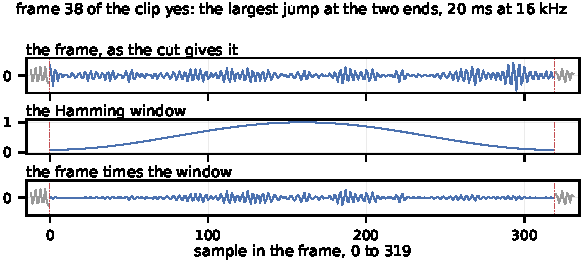
\includegraphics[width=0.86\textwidth]{images/modules/MC-5/mc5_window.pdf}
  \par\endgroup
  \vskip 0.2em
  \small
  \begin{itemize}
    \item A frame starts and ends in the middle of the sound. The jump at
          each end looks like a high frequency that is not there.
    \item The Hamming window multiplies the frame by a curve that is 1 in
          the middle and close to 0 at the two ends.
    \item It removes the jump, and it removes a little resolution. A
          longer frame resolves better and says less about the time.
  \end{itemize}
\end{frame}

% --------------------------------------------------------- 8. the FFT
\begin{frame}{Step 4: the FFT and the power}
  \begin{itemize}
    \item The FFT of a frame of 320 values with 512 points gives 257 bins.
    \item The bins are 31.25 Hz apart, and bin 0 is the direct current.
    \item The power spectrum is the square of the magnitude:
          $P(f) = |X(f)|^2$. Squaring lifts the strong frequencies over the
          weak ones.
  \end{itemize}
  \vskip 0.4em
  \small The frame is shorter than the FFT, so the FFT pads it with 192
  zeros. The bins then sit closer than the frame can resolve, and the curve
  is smoother. The resolution stays that of 20 ms, which is 50 Hz.
  \source{"Machine Learning Systems", chapter "KWS Feature Engineering",
    the steps "FFT" and the note on the power spectrum.}
\end{frame}

% -------------------------------------------------------- 9. the Mel scale
\begin{frame}{The Mel scale}
  \begin{equation*}
    \text{mel}(f) = 2595 \log_{10}\left(1 + \frac{f}{700}\right)
  \end{equation*}
  \small
  \begin{itemize}
    \item 1000 Hz on the linear scale is 1000 mel. 1000 Hz on the Mel scale
          is 1500 mel, and 3000 Hz is 2000 mel.
    \item The ear hears the difference between two low tones better than the
          difference between two high tones of the same width in hertz.
    \item So the filters of the bank are narrow at the bottom and wide at
          the top. With 32 filters from 0 to 8000 Hz, the first is about
          60 Hz wide and the last about 660 Hz.
  \end{itemize}
  \vskip 0.3em
  \small The number of filters is a choice. The chapter recommends 20 to 40
  triangles.
  \source{The Mel scale and the number of filters, from "Machine Learning
    Systems", chapter "KWS Feature Engineering", the steps "Mel Filter
    Banks" and the section "Computing MFCCs". The two widths are the value
    of the lab of this module.}
\end{frame}

% ------------------------------------------------------- 10. the bank
\begin{frame}{Step 5: the filter bank and the logarithm}
  \begingroup\centering
  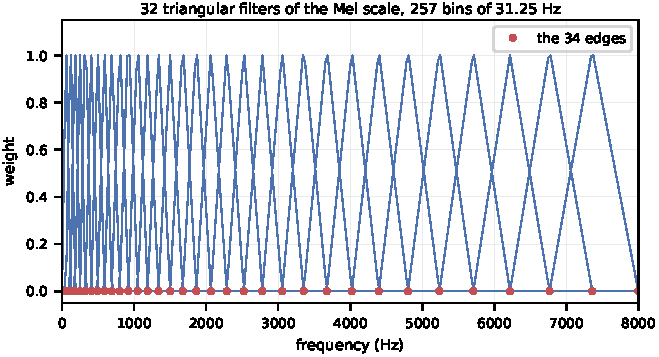
\includegraphics[width=0.90\textwidth]{images/modules/MC-5/mc5_melbank.pdf}
  \par\endgroup
  \vskip 0.2em
  \small Each filter is a triangle that rises from 0 to 1 and falls back to
  0. Two filters touch at their half point, so no frequency is lost. The
  energy of one filter is the sum of the power of the bins under it.
  \vskip 0.2em
  \small The logarithm comes next: it turns the wide dynamic range of
  audio into a range that a network can work with.
\end{frame}

% ------------------------------------------------------- 11. the cepstrum
\begin{frame}{Step 6: the cosine transform}
  \begin{equation*}
    c[k] = \sum_{m=0}^{N-1} \log E[m]
      \cos\left(\frac{\pi k (2m + 1)}{2N}\right)
  \end{equation*}
  \small
  \begin{itemize}
    \item The cosine transform mixes the 32 log energies of a frame into 13
          numbers.
    \item The first coefficient is the mean of the 32 values, so it holds
          the energy of the frame.
    \item The other coefficients describe the shape of the spectrum: the
          first ones the envelope, the last ones the fine structure.
    \item Mixing decorrelates the values, so the network sees numbers that
          do not repeat one another.
  \end{itemize}
  \vskip 0.3em
  \small The chapter keeps the first 12 or 13 coefficients and drops the
  rest.
  \source{"Machine Learning Systems", chapter "KWS Feature Engineering",
    the step "Discrete Cosine Transform (DCT)".}
\end{frame}

% ------------------------------------------------------ 12. three forms
\begin{frame}{One second of audio in three forms}
  \begingroup\centering
  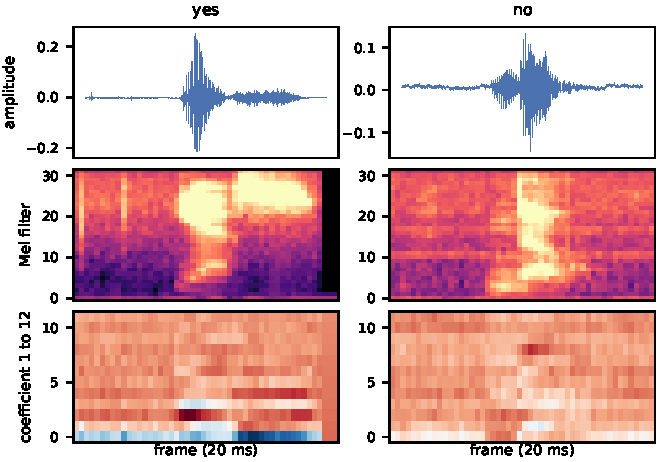
\includegraphics[width=0.78\textwidth]{images/modules/MC-5/mc5_features.pdf}
  \par\endgroup
  \vskip 0.1em
  \small The top row is the waveform, the middle row the energy of the 32
  filters for the 50 frames, and the bottom row the coefficient 1 to 12 of
  each frame. The first coefficient is not drawn: it is the energy.
\end{frame}

% ------------------------------------------------------ 13. the sizes
\begin{frame}{What each step does to the number of values}
  \footnotesize
  \setlength{\tabcolsep}{4pt}
  \begin{tabular}{@{}L{3.4cm}L{2.6cm}L{3.6cm}@{}}
    \toprule
    After & Values per frame & What it is \\
    \midrule
    The samples & 16000 & one second, no frame \\
    The framing & 320 & 20 ms of samples \\
    The FFT & 257 & one value per bin \\
    The Mel filters & 32 & the energy of each filter \\
    The logarithm & 32 & the energy in a decibel scale \\
    The cosine transform & 13 & the cepstral coefficients \\
    \bottomrule
  \end{tabular}
  \vskip 0.5em
  \small
  \begin{itemize}
    \item A clip of 1 s has 50 frames, so it gives $50 \times 13 = 650$
          values instead of 16000. The pipeline divides the number of
          values by 24.6.
    \item Only two steps reduce the number of values: the filters and the
          cosine transform.
  \end{itemize}
\end{frame}

% --------------------------------------------------- 14. the comparison
\begin{frame}{The cepstrum against the spectrogram}
  \begingroup\centering
  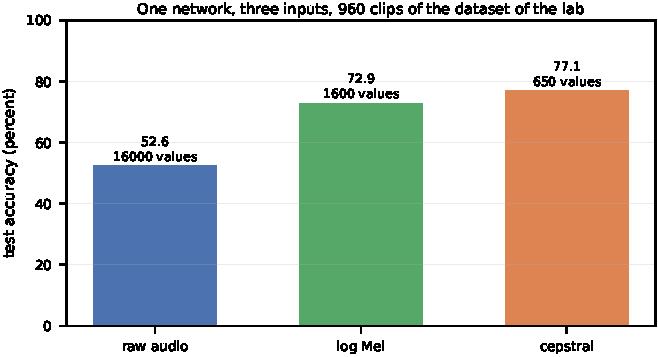
\includegraphics[width=0.88\textwidth]{images/modules/MC-5/mc5_inputs.pdf}
  \par\endgroup
  \vskip 0.2em
  \small One network, three inputs, the same 768 training clips. The
  cepstrum wins on all three counts: the fewest values, the fewest
  parameters, and the best test accuracy.
  \vskip 0.2em
  \small The raw audio needs 25 times more values than the cepstrum, 142
  times more parameters, and it does not learn with this little data.
\end{frame}

% ------------------------------------------------------- 15. when to use
\begin{frame}{When the spectrogram is the better choice}
  \begin{columns}[T]
    \begin{column}{0.48\textwidth}
      \small\textbf{The cepstrum is stronger for}
      \begin{itemize}
        \item speech and keywords,
        \item the identity of a speaker,
        \item the emotion of a voice,
        \item a device with little memory.
      \end{itemize}
    \end{column}
    \begin{column}{0.48\textwidth}
      \small\textbf{The spectrogram is stronger for}
      \begin{itemize}
        \item music and the instruments in it,
        \item rain, wind, and traffic,
        \item the calls of birds,
        \item finding a click in a recording.
      \end{itemize}
    \end{column}
  \end{columns}
  \vskip 0.4em
  \small The cepstrum keeps the envelope of the spectrum and drops its fine
  structure, so it is stable against the noise and against a change of
  loudness. A task that lives in the fine structure needs the whole
  spectrum.
  \source{"Machine Learning Systems", chapter "KWS Feature Engineering",
    the sections "MFCCs are particularly strong for" and "Spectrograms or
    MFEs are often more suitable for".}
\end{frame}

% ---------------------------------------------------- 16. what to remember
\begin{frame}{What to remember}
  \small
  \begin{enumerate}
    \item One second of audio at 16 kHz is 16000 values. The model must not
          read them.
    \item Six steps: the pre-emphasis, the framing, the window, the FFT, the
          Mel filters with the logarithm, and the cosine transform.
    \item The Mel scale gives the low frequencies more filters, because the
          ear resolves them better.
    \item The cosine transform is the only step that reduces the number of
          values by a large factor: 32 energies become 13 coefficients.
    \item Choose between the cepstrum and the spectrogram from the task,
          and check the choice with a measurement.
  \end{enumerate}
\end{frame}

% ------------------------------------------------------------- exercise
\exerciseframe{Count the values}{A device samples at 16 kHz, cuts the signal
into frames of 20 ms with the same stride, uses an FFT of 512 points, 32
triangular filters of the Mel scale, and keeps 13 cepstral coefficients.

\begin{enumerate}
  \item How many values does one second of audio give before the pipeline,
        and after it?
  \item How many multiply-accumulate operations does the first convolution
        of the lab network need for one clip, with 16 filters of 3 frames
        and 13 input values?
  \item Name the step that reduces the number of values the most.
\end{enumerate}
}

\answerframe{Count the values}{
  \begin{enumerate}
    \item Before: 16000 samples. After: a clip of 1 s has
          $1 + (16000 - 320)/320 = 50$ frames, and each frame gives 13
          values, so $50 \times 13 = 650$ values. The pipeline divides the
          number of values by 24.6.
    \item A convolution with 3 frames and no padding leaves
          $50 - 2 = 48$ positions. Each position needs
          $3 \times 13 \times 16 = 624$ multiply-accumulate operations, so
          the layer needs $48 \times 624 = 29952$ operations for one clip.
    \item The cosine transform, which turns the 32 log energies of a frame
          into 13 coefficients. The FFT raises the number of values from
          320 to 257 before the filters, and the filters keep 32.
  \end{enumerate}
  \vskip 0.3em
  \small Part 2 assumes the network of the lab, with valid convolutions.
  A convolution with a padding of `same` would keep the 50 positions and
  need 31200 operations.
}
% A module of type T+L keeps the lab part. A module of type T deletes the
% next line and the file lab.tex.
% Lab part of the module.
%
% Module MC-5 of Section 6.1 of the syllabus: "Keyword spotting features and
% training in Python". Type T+L, 90 minutes: about 45 minutes of theory and
% 45 minutes of lab. The lab needs no board. It runs on a laptop CPU and
% needs the public dataset of Edge Impulse, which a script of the folder
% downloads.
%
% The parts follow the README of the lab folder. The frames show the form of
% the output and the values that check the method. No value here is a
% measurement of a board.

% --------------------------------------------------------------- 1. the goal
\begin{frame}{Lab: goal and plan}
  \small
  \begin{itemize}
    \item \textbf{Goal.} You compute the cepstral coefficients of a clip of
          one second with numpy only, and you train a small classifier on
          them, with no tool of Edge Impulse Studio.
    \item \textbf{Deliverable.} The table of section 10 of the notebook,
          copied into \code{report.md}, and the answers of its three questions.
  \end{itemize}
  \vskip 0.5em
  \footnotesize
  \setlength{\tabcolsep}{4pt}
  \begin{tabular}{@{}L{1.0cm}L{7.2cm}L{1.5cm}@{}}
    \toprule
    Part & Content & Time \\
    \midrule
    A & The clips, and the triangular filters of the Mel scale & 12 min \\
    B & The cepstral coefficients, and the plot of one clip & 13 min \\
    C & The classifier, and its number of parameters & 8 min \\
    D & Three inputs for the same task & 12 min \\
    \bottomrule
  \end{tabular}
  \vskip 0.5em
\end{frame}

% ---------------------------------------------------------- 2. the dataset
\begin{frame}{Lab: the dataset}
  \small
  \begin{itemize}
    \item The script \code{host/get\_keywords.py} downloads the file
          \code{keywords2.zip} of Edge Impulse (139 MB) into the folder
          \code{downloads/}, one time. Then it writes 240 clips of each of
          the four classes into \code{keywords/clips/}.
    \item The four classes are \code{no}, \code{noise}, \code{unknown}, and
          \code{yes}. Each clip has 1 s of audio at 16 kHz.
    \item The notebook reads the amplitudes from text files, so it needs no
          audio package.
  \end{itemize}
  \vskip 0.5em
  \begin{center}
  \begin{tabular}{@{}lrrr@{}}
    \toprule
    Class & Clips & Training & Test \\
    \midrule
    \code{no} & 240 & 192 & 48 \\
    \code{noise} & 240 & 192 & 48 \\
    \code{unknown} & 240 & 192 & 48 \\
    \code{yes} & 240 & 192 & 48 \\
    \bottomrule
  \end{tabular}
  \end{center}
  \small The split is random, so a clip of one speaker can be in both sets.
  The notebook says so in section 6.
\end{frame}

% ------------------------------------------------------------- 3. the files
\begin{frame}{Lab: files}
  \small
  \setlength{\tabcolsep}{4pt}
  \begin{tabular}{@{}L{3.9cm}L{5.3cm}@{}}
    \toprule
    File & Content \\
    \midrule
    \code{mfcc\_training.ipynb} & The notebook. It has four tasks. \\
    \code{host/get\_keywords.py} & Downloads the dataset. \\
    \code{report.md} & The report to hand in. \\
    \code{solutions/} & The notebook with all tasks complete and with its
      output, and an example report. \\
    \code{TEST\_NOTES.md} & The code status and the steps to run the lab. \\
    \bottomrule
  \end{tabular}
  \vskip 0.5em
  \small
  \begin{itemize}
    \item Section 2 of the notebook gives the functions of the pipeline that
          need no decision from you. Two of the four tasks use them.
    \item Section 6 caches the features in the file \code{features.npz}, so
          the second run of the notebook is fast.
  \end{itemize}
\end{frame}

% ---------------------------------------------------------------- 4. part A
\begin{frame}[fragile]{Part A: the clips and the filter bank (12 min)}
  \small
  \begin{enumerate}
    \item Get the dataset, one time, from the folder of the lab:
\begin{lstlisting}[style=shell]
python3 host/get_keywords.py
\end{lstlisting}
    \item Start Jupyter from the folder of the lab, and run sections 0 and 1.
    \item \textbf{Task 1.} Write \code{mel\_filters(n\_filters, n\_bins,
          f\_min, f\_max, sample\_rate)}: the matrix of the 32 triangular
          filters of the Mel scale.
    \item Run the cell after the task.
  \end{enumerate}
  \vskip 0.4em
  \small You see the peak of the first filter at bin 2 and of the last one
  at bin 236. The first filter is 3 bins wide and the last one 40 bins wide.
  That is the Mel scale: narrow at the bottom, wide at the top.
\end{frame}

% ---------------------------------------------------------------- 5. part B
\begin{frame}{Part B: the cepstral coefficients (13 min)}
  \small
  \begin{enumerate}
    \item \textbf{Task 2.} Write \code{mfcc(clip, filters=None)}: the
          pre-emphasis, the framing, the Hamming window, the FFT, the
          filters, the logarithm, and the cosine transform.
    \item Run the cell after the task. Then run section 5.
    \item Look at the three panels. Write in the report what the middle
          panel shows and what the bottom panel shows.
    \item Run section 6. Write the run time of the features in the report.
  \end{enumerate}
  \vskip 0.4em
  \small The notebook prints the mean of the first coefficient, which is
  $-13.071$, and the mean of the last one, which is $0.064$. The first
  coefficient is large because it holds the energy of the frame, and the
  logarithm of a small power is a large negative number.
\end{frame}

% ---------------------------------------------------------------- 6. part C
\begin{frame}{Part C: the classifier (8 min)}
  \small
  \begin{enumerate}
    \item \textbf{Task 3.} Write \code{make\_model(n\_frames, n\_features)}:
          two \code{Conv1D} layers with 16 and with 32 filters of 3 frames,
          each with a max pooling of 2, then a \code{Dense} layer with 4
          outputs.
    \item Run the cell after the task. The check calculates the expected
          number of parameters itself, with the length that each
          convolution and each pooling layer leaves.
    \item Run the next cell to train the model.
  \end{enumerate}
  \vskip 0.5em
  \begin{center}
  \begin{tabular}{@{}l@{}}
    \toprule
    the input has 50 frames of 13 values, and 11 frames after the two \\
    convolutions and the two pooling layers \\
    parameters 3620 (expected 3620), outputs 4 \\
    the cepstral coefficients: 650 values per clip, 3620 parameters, \\
    test accuracy 77.1 percent \\
    \bottomrule
  \end{tabular}
  \end{center}
\end{frame}

% ---------------------------------------------------------------- 7. part D
\begin{frame}{Part D: three inputs for the same task (12 min)}
  \small
  \begin{enumerate}
    \item \textbf{Task 4.} Before you run the next cell, complete
          \code{values\_per\_clip} with the number of values that one clip
          gives for each of the three inputs, and write in
          \code{best\_input} the input that you expect to win.
    \item Run the next cell and section 10, and copy the table into the
          report.
    \item Answer the three questions of the notebook.
  \end{enumerate}
  \vskip 0.4em
  \small The three lines of the notebook: the raw audio has 16000 values
  and 513380 parameters, the log Mel spectrogram 1600 values and 4532
  parameters, and the cepstral coefficients 650 values and 3620 parameters.
\end{frame}

% ------------------------------------------------------------ 8. the check
\begin{frame}{Check criterion and Decision Log}
  \small
  \begin{itemize}
    \item The notebook prints \code{complete} for tasks 1, 2, 3, and 4.
    \item The table of the report has three rows, each with the number of
          values, the number of parameters, and a measured test accuracy.
    \item The three questions of the report have answers with numbers from
          your own run.
    \item The Decision Log names one decision and one number.
  \end{itemize}
  \vskip 0.5em
  \keypoint{Question of the Decision Log: the device must say one word every
    500 ms on a battery. Which of the three inputs do you put in the
    firmware, and which number of your table decides it?}
\end{frame}

% ------------------------------------------------------- 9. common problems
\begin{frame}{Common problems}
  \small
  \setlength{\tabcolsep}{3pt}
  \begin{tabular}{@{}L{4.0cm}L{5.2cm}@{}}
    \toprule
    Problem & Fix \\
    \midrule
    The notebook stops with \code{No clip in the folder} & Run
      \code{host/get\_keywords.py} first. The download is 139 MB. \\
    \code{Task 1} says that the last filter must reach bin 205 & A bin is
      \code{frequency * nfft / sample\_rate}, and \code{nfft} is
      \code{2 * (n\_bins - 1)}. \\
    \code{Task 2} says that the answer needs 50 rows & A clip of 16000
      samples at a stride of 320 gives 50 frames. Return one row for each. \\
    \code{Task 3} says that the model raises an error & A layer is missing,
      or a layer was added with a tensor instead of with its input. \\
    The plot of section 5 is empty & Delete \code{features.npz} and run
      section 6 again. \\
    The notebook is slow & The first run computes the features of 960
      clips. The file \code{features.npz} makes the next run fast. \\
    \bottomrule
  \end{tabular}
  \vskip 0.5em
  \small The README of the lab folder has the full list of the checks of the
  notebook and the run time.
\end{frame}
% Credits frame. Section 10 of the syllabus gives this text.
% Each deck ends with this frame:
%   % Credits frame. Section 10 of the syllabus gives this text.
% Each deck ends with this frame:
%   % Credits frame. Section 10 of the syllabus gives this text.
% Each deck ends with this frame:
%   \input{sections/credits}
%
% The list \coursecredits selects the sources. preamble/course.tex gives the
% default list and one command for each source. The main file of a deck
% changes the list before it inputs this file, so that the frame names only
% the sources that the deck uses:
%   \renewcommand{\coursecredits}{\creditmlsys\creditxiao}
\begin{frame}[allowframebreaks]{Credits}
  \vskip 0.6em
  \begin{itemize}\footnotesize\itemsep 0.4em
    \coursecredits
  \end{itemize}
  \vskip 0.8em
\end{frame}

%
% The list \coursecredits selects the sources. preamble/course.tex gives the
% default list and one command for each source. The main file of a deck
% changes the list before it inputs this file, so that the frame names only
% the sources that the deck uses:
%   \renewcommand{\coursecredits}{\creditmlsys\creditxiao}
\begin{frame}[allowframebreaks]{Credits}
  \vskip 0.6em
  \begin{itemize}\footnotesize\itemsep 0.4em
    \coursecredits
  \end{itemize}
  \vskip 0.8em
\end{frame}

%
% The list \coursecredits selects the sources. preamble/course.tex gives the
% default list and one command for each source. The main file of a deck
% changes the list before it inputs this file, so that the frame names only
% the sources that the deck uses:
%   \renewcommand{\coursecredits}{\creditmlsys\creditxiao}
\begin{frame}[allowframebreaks]{Credits}
  \vskip 0.6em
  \begin{itemize}\footnotesize\itemsep 0.4em
    \coursecredits
  \end{itemize}
  \vskip 0.8em
\end{frame}


\end{document}